
\section{Introduction}
\label{sec:intro}

\kbf{Some of these paragraphs may need to be shuffled a bit, order may not be the
most logical}

\kbf{Following paragraph is nearly identical to parallel submission}
\sll{First paragraph is very close to SC18 paper.  I'm not sure the logic holds up.
CEs are arguably \emph{more} likely with Chipkill than SECDED.}

Maintaining the performance of high-performance computing~(HPC) applications as
failures become more and more frequent is a major challenge that needs to be
addressed for next-generation extreme-scale systems.  Many recent studies have
demonstrated that hardware failures are expected to become ever more
common~\cite{Bergman08exascalecomputing}.  Increasing the scale of HPC systems
requires the aggregation of larger number of individual components.  More
components means more frequent failures.  Current systems use powerful
error-correcting codes~(ECC), e.g., chipkill-correct, to protect against DRAM
errors.  However, chipkill-correct (and other similar techniques) require the
activation of a large number of memory devices (four times more than
less-protective techniques like single error correct double error
detect~(SECDED))~\cite{Jian13}.  Activating more memory devices requires more
power for each memory access.  However, because of tightening power budgets on
next-generation systems~\cite{Bergman08exascalecomputing} and technology
changes like High-Bandwidth Memory~(HBM)~\cite{HBM}, it is not yet clear that
chipkill-correct will continue to be viable.  Reduced device-feature sizes also
have the potential to result in more frequent failures.  Understanding the
implications of these trends requires that we have detailed knowledge of how
failures affect current leadership-class systems.

\sll{This is pretty detailed to include in the introduction.  Maybe a background
section?}
Error detection and handling is critical to pinpointing failing components and
taking corrective action in a timely fashion.  Error handling is typically
a cooperative activity between the platform hardware, firmware (UEFI or BIOS),
and the host operating system.  Errors are signaled in host firmware
or the OS directly. The firmware reads the hardware registers (\sll{of the CPU??}) 
and analyzes the component that generated the error in an effort to assess the severity of
the error.  Firmware then creates a detailed description of the error and
notifies the OS of its occurrence. Additionally, the host firmware (\sll{is ``firmware''
different than ``host firmware''}) may communicate
this error to the baseboard management controller~(BMC) for system management purposes.
When the error notification is signaled to the OS, either directly or from host
firmware, the OS typically inspect hardware registers or firmware and initiate
corrective action.  Time spent handling an error by the OS and/or firmware can perturb
application progress, even in cases where the failure does not initiate a
restart.

\sll{I \emph{think} that we're really only talking about memory errors?  Can we say that?}
Errors are typically classified into three categories: Correctable,
Uncorrectable, and Fatal. Correctable errors (CE) are errors that can be
corrected or mitigated in hardware such that the platform's state is the same as it
would have been left if no error had occurred.  An example of a CE is is a single bit 
(or single symbol in the case of chipkill) error.  Detected, uncorrectable errors (DUE) are those
errors that could be detected by hardware, but could not be corrected.
Multi-bit/Multi-symbol errors are an example of such an error.  In many cases
it is possible for the system to continue functioning in the face of these
errors, perhaps with a certain amount of lost state.  \sll{Not sure what the ``In many
cases'' caveat means.  If it can't continue functioning then isn't it a \emph{fatal}
error?}  Finally, fatal errors corrupt the state of the platform such that continued 
correct operation can no longer be guaranteed.  Recovering from a fatal error typically 
requires a full system halt and a reboot.

Recent research has largely focused on uncorrectable and fatal errors: errors
that require applications to be restarted.  However, the impacts of the most common
type of errors in large-scale systems, correctable errors, have largely been overlooked. An
analysis of failures on recent leadership-class systems shows that the
correctable failure rates vary from a factor of
8~\cite{siddiqua:2017:lifetime,levy:2018:lessons} to a factor of
20~\cite{meza:2015:revisiting} times more frequent than uncorrectable errors.
\sll{Can we say this?  Isn't this getting at the data that AMD required us to remove?}
Correctable errors are typically handled at a hardware level and are largely invisible 
to the application.  While the application can continue to make progress despite the
presence of correctable errors (i.e. restarting the application is unnecessary), the 
time required to correct and log these errors has the potential to impact application
performance by delaying application computation. These CEs can be transient,
generating only one or a small handful of error events on a node, or can be
persistent and generate in some cases millions of error events.  \sll{Struggling with
the significance of the difference between transient and persistent CEs.}  These
\emph{bursty} CE events can lead to significant application slowdowns even on
current systems~\cite{BURSTY}.  \sll{\emph{bursty} still feels out of place to me.  Fundamentally,
we only care about rates, not about whether there are ``bursts'' of errors.  It's also not
clear to me from this paragraph what we mean by ``bursty''.}

\let\workinterval\relax
\let\ckpttime\relax
\let\txdelay\relax
\let\msgtime\relax
\let\minheight\relax
\newcommand{\workinterval}{1.25cm}
\newcommand{\ckpttime}{0.625cm}
\newcommand{\txdelay}{2.0mm}
\newcommand{\msgtime}{\workinterval+\txdelay}
\newcommand{\minheight}{0.5cm}
\usetikzlibrary{positioning}

\tikzstyle{position}=[fill=none,text=white,draw=none]
\tikzstyle{proc}=[fill=none,text=black,draw=none,shape=rectangle]
\tikzstyle{origtotal}=[fill=none,text=black,draw=black,shape=rectangle,
                       minimum width=3*\workinterval+2*\txdelay,
                       minimum height=\minheight]
\tikzstyle{coordtotal}=[fill=none,text=black,draw=black,shape=rectangle,
                        minimum width=3*\workinterval+\ckpttime+2*\txdelay,
                        minimum height=\minheight]
\tikzstyle{uncoordtotal}=[fill=none,text=black,draw=black,shape=rectangle,
                          minimum width=3*\workinterval+2*\ckpttime+2*\txdelay,
                          minimum height=\minheight]
\tikzstyle{ckpt}=[fill=black,text=white,draw=none,shape=rectangle,
                  minimum width=\ckpttime,minimum height=\minheight]
\tikzstyle{stall}=[fill=black!20,text=white,draw=black,shape=rectangle,
                   minimum height=\minheight]

\begin{figure*}[bt]
\centering{
\subfloat[without CE activity]{
\resizebox{0.25\textwidth}{!}{
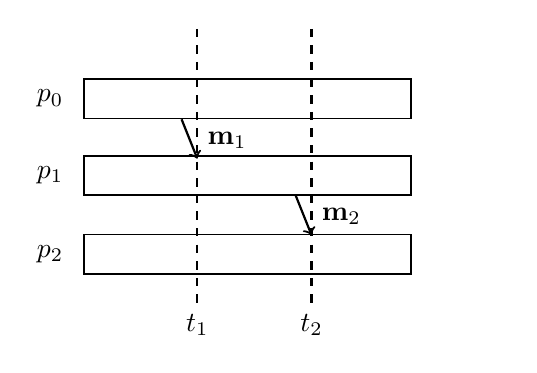
\begin{tikzpicture}[semithick]

\node [proc] (p0) {$p_0$};
\node [position, right= 0.125cm of p0, minimum width=3*\workinterval+2*\ckpttime+2*\txdelay] (n0) {};
\node [origtotal, right= 0.125cm of p0]  (v1) {};
\node [position, right= \msgtime of v1.north west ]  (v2) {};
\node [position, right= \msgtime of v2.west ]  (v4) {};

\node [proc, below = 5mm of p0] (p1) {$p_1$};
\node [origtotal, right= 0.125cm of p1]  (v5) {};
\node [position, right= \msgtime of v5.west ]  (v6) {};
\node [position, right= \workinterval of v6.south west ]  (v8) {};

\node [proc, below of=p1] (p2) {$p_2$};
\node [origtotal, right= 0.125cm of p2]  (v9) {};
\node [position, right= \msgtime of v9.west ]  (v10) {};
\node [position, right= \msgtime of v10.west ]  (v11) {};

\draw [->, thick] (v1.south west) ++(\workinterval,0) -- ++(\txdelay, -5.00mm) 
      node[above right] {$\mathbf{m}_1$};
\draw [->, thick] (v8.south west) -- ++(\txdelay, -5.00mm) node[above right] {$\mathbf{m}_2$};

\draw [thick, dashed] (v2.north west) ++(0.0cm, 5.0mm) -- (v10.south west) -- ++(0, -5.0mm) node[below] {$t_1$};
\draw [thick, dashed] (v4.north west) ++(0.0cm, 5.0mm) -- (v11.south west) -- ++(0, -5.0mm) node[below] {$t_2$};
\end{tikzpicture} 
}\label{subfig:no_ckpt}
}
%
%
%\subfigure[uncoordinated checkpointing]{
\subfloat[with local CE activity delays]{
\resizebox{0.25\textwidth}{!}{
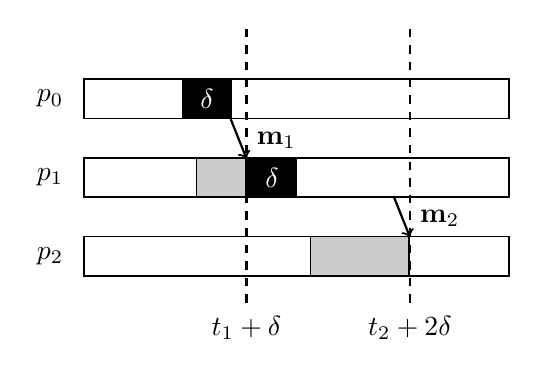
\begin{tikzpicture}[semithick]

\node [proc] (p0) {$p_0$};
\node [uncoordtotal, right= 0.125cm of p0]  (v1) {};
\node [position, right= \msgtime+\ckpttime of v1.north west ]  (v2) {};
\node [ckpt, right= \workinterval of v1.west ]  (v3) {$\delta$};
\node [position, right= \msgtime+\ckpttime of v2.west ]  (v4) {};

\node [proc, below of=p0] (p1) {$p_1$};
\node [uncoordtotal, right= 0.125cm of p1]  (v5) {};
\node [position, right= \msgtime+\ckpttime of v5.west ]  (v6) {};
\node [stall, minimum width=\ckpttime, left= 0.0cm of v6.west ]  (v7) {};
\node [ckpt, right= 0.00cm of v6.west ]  (v7) {$\delta$};
\node [position, right= \workinterval+\ckpttime of v6.south west ]  (v8) {};

\node [proc, below of=p1] (p2) {$p_2$};
\node [uncoordtotal, right= 0.125cm of p2]  (v9) {};
\node [position, right= \msgtime+\ckpttime of v9.west ]  (v10) {};
\node [position, right= \msgtime+\ckpttime of v10.west ]  (v11) {};
\node [stall, minimum width=2*\ckpttime, left= 0.00cm of v11.west ]  (v12) {};

\draw [->, thick] (v1.south west) ++(\workinterval+\ckpttime,0) -- ++(\txdelay, -5.00mm) 
      node[above right] {$\mathbf{m}_1$};
\draw [->, thick] (v8.south west) -- ++(2.0mm, -5.00mm) node[above right] {$\mathbf{m}_2$};

\draw [thick, dashed] (v2.north west) ++(0.0cm, 5.0mm) -- (v10.south west) -- ++(0, -5.0mm) node[below] {$t_1+\delta$};
\draw [thick, dashed] (v4.north west) ++(0.0cm, 5.0mm) -- (v11.south west) -- ++(0, -5.0mm) node[below] {$t_2+2\delta$};
\end{tikzpicture} 
}\label{subfig:uncoord_ckpt}
}
}
\caption{
        Example of how delays introduced by local correctable error (CE)
        activities may propagate along application communication dependencies.
        The processes $p_1$, $p_2$, and $p_3$ exchange two messages $m_1$ and
        $m_2$ in each of the three scenarios. The black regions marked with a
        white $\delta$ denote the execution of CE mitigation activities.  The
        grey regions denote periods in which the execution of a process is
        stalled due to an unsatisfied communication dependency.
}\label{fig:propagation}
\end{figure*}


In this paper, we present a detailed analysis of the relationship between the cost of
correcting and logging memory CEs and application performance on large-scale systems.
Specifically, to better understand the potential performance impact of CEs, we answer the 
following key questions:

\begin{itemize}
  \item What is the expected performance impact of CEs on applications running on current and 
        projected future extreme-scale systems?
  \item How frequently can CEs occur without significantly degrading application performance?
  \item What is the application performance impact of CEs that are isolated to a single process?
  \item How can system designers address CEs to improve application performance on next-generation systems?
\end{itemize}
\sll{For reference, these are the existing questions.}
\begin{itemize}
        \item At what CE frequency does one "Bursty" node have significant
              performance impact on current and future systems?
        \item Given current correctable error rates, what is the performance
              overheads of CE on current and expected future extreme-scale systems?
        \item How much can CE rates increase without significantly impacting
              performance?
        \item Given these performance overheads, what advice can we give system
              designers to keep slowdowns due to CEs low?
\end{itemize}

We anticipate that the relationship between application performance and CE 
overheads will become increasingly more important as error rates increase on
next-generation extreme-scale systems.  Dramatic growth in system size (both
in terms of node count and node density) and total memory volume are likely
to lead to more frequent CEs on future systems. 
\kbf{beef up justification for following sentence to justify increased rates}
Additionally, smaller feature sizes, manufacturing variability, changing memory
protection technology, hardware aging effects, and sub-threshold logic have the
potential to further increase the rate of CEs.  
More specifically, using a wide array of
applications, we demonstrate that the overheads associated with  correctable
errors can have a significant impact on overall application performance.  These
local correctable errors introduce overheads that can amplified or absorbed
globally by an application depending on an application's communication
activities. \sll{These last two sentences seem to be repeating content from 
elsewhere in the section.}

The introduction of delays in application processes by CE-related correction and 
logging activities is analogous to how operating system noise (or \emph{jitter}) can 
affect the performance of large-scale applications~\cite{Hoefler:2010:Characterizing, 
Ferreira:08:characterizing}.  \Cref{fig:propagation} illustrates this phenomenon.  
\Cref{subfig:no_ckpt} shows a simple application running across three processes 
($p_0$, $p_1$, and $p_2$) in the absence of CEs.  These three processes exchange two 
messages, $\mathbf{m}_1$ and $\mathbf{m}_2$.  For the purposes of this figure, we assume 
that these messages represent strict dependencies: any delay in the arrival of a message requires the
recipient to stall until the message is received. \Cref{subfig:uncoord_ckpt}
illustrates the potential impact of CE correction and logging.  If $p_0$
encounters a CE at the instant before it would have otherwise sent $\mathbf{m}_1$,
then $p_1$ is forced to wait (the waiting period is shown in grey) until the
message arrives.  If $p_1$ subsequently encounters a CE before sending
$\mathbf{m}_2$, then $p_2$ is forced to wait.  Part of the time that $p_2$
spends waiting is due to a delay that was originated by $p_0$, which it does not
communicate with.  The key point is that delays due to CEs can propagate based on 
communication dependencies in the application.

Based on the studies presented in this paper, we make the following
contributions \kbf{Contributions need revisiting}:
\sll{Do we need contributions?  It seems like we should include either the
questions above or the contributions below.}

\begin{itemize}

\item we demonstrate the impacts of the hardware/firmware/OS activities
        associated with correctable errors, and how those activities can changes
        based on platform configuration \S{?};

\item we analyze the potential impacts of this correctable errors on application
        performance.  We demonstrate that he performance impact of logging
                correctable DRAM errors is modest at error rates observed on
                current system.  In addition, we show these impacts change with
                increased error rates \S\S{?};

\item we show how an application's scale and communication pattern can dictate
        whether local overheads due to correctables are amplifies or absorbed by
        other processes \S\S{?}; and

\item we show the interplay between the correctable error rate and the duration
        of each mitigation activity, providing prescriptive advice on how best
        to reduce overheads due to these common errors on leadership-class platforms
        \S{?}.

\end{itemize}

Overall, this work provides critical analysis and insight into the overheads of
common correctable errors and provides practical advice to users and systems
administrators in an effort to fine-tune performance to application and system
characteristics.
